\section{伽利略相对性原理与狭义相对论}

\subsection{惯性系与经典变换}

惯性系是自由质点保持静止或匀速直线运动的参考系。伽利略相对性原理指出，力学规律在所有惯性系中具有相同形式。若 $S'$ 相对 $S$ 沿 $+x$ 以速度 $V$ 匀速运动，且两原点在零时刻重合，经典运动学采用
\[
x'=x-Vt,\quad y'=y,\quad z'=z,\quad t'=t,
\qquad u'_x=u_x-V.
\]
这里的绝对时间使速度直接相减。当 $u_x=c$ 时，式中会给出 $c-V$，不能同时满足所有惯性系中真空光速均为 $c$ 的要求。

狭义相对论采用两条基本原理：所有惯性系中的物理定律具有相同形式；所有惯性系测得的真空光速均为 $c$，与光源的运动无关。以下取 $c=3.00\times10^8\,\mathrm{m/s}$。介质中的光速仍须注明介质的静止系。

光速不变改变的是不同惯性系的时空坐标转换。应用之前，须先明确这些坐标由怎样的测量给出。

低速极限下，相对论变换回到经典变换，说明经典关系在日常低速范围内仍是良好近似。判据涉及相关运动速度与 $c$ 的比值；对于光本身，即使光源或装置运动很慢，也不能先把光速按伽利略规则相减。介质内传播还要明确介质静止系，不能把真空光速不变直接改写为所有参考系中的介质光速相同。

\subsection{事件与时空间隔}

事件由确定的地点和时刻描述，例如粒子产生、炸弹爆炸或闪光到达探测器。一个惯性系用静止尺和分布在各处的同步钟记录坐标，而眼睛接收到光的时刻还包含信号传播时间。改变参考系时，必须变换同一事件的位置和时刻，不能把远处“发生”与眼前“收到”当成一个事件。

两事件的间隔定义为
\begin{equation}\label{eq:hrinterval}
\Delta s^2=c^2\Delta t^2-\Delta x^2-\Delta y^2-\Delta z^2.
\end{equation}
洛伦兹变换保持这一量不变。$\Delta s^2>0$ 为类时间隔，可以由亚光速物体连接；$\Delta s^2=0$ 为类光间隔；$\Delta s^2<0$ 为类空间隔，不能用不超光速的信号连接。
\fig{fig:hrcone}{横轴 $\Delta x$ 与纵轴 $c\Delta t$ 等比例。真空光线斜率为 $\pm1$，类时事件位于光锥内部。}{
\begin{tikzpicture}[scale=.85]
\draw[axis](-3.5,0)--(3.7,0)node[right]{$\Delta x$};\draw[axis](0,-.3)--(0,4.2)node[above]{$c\Delta t$};
\fill[black!6](0,0)--(3.5,3.5)--(-3.5,3.5)--cycle;\draw[light](0,0)--(3.5,3.5);\draw[light](0,0)--(-3.5,3.5);
\node at(0,2.6){未来类时区域};\node at(3,.8){类空};\node at(-3,.8){类空};\node[below left]at(0,0){$O$};
\end{tikzpicture}}

若要把两事件间的时间差解释为随身钟的走时，须先确认它们在同一物体的世界线上。对匀速运动，$\Delta\bm r=\bm u\Delta t$，故
\[
c^2\Delta\tau^2=c^2\Delta t^2-|\Delta\bm r|^2,
\qquad \Delta\tau=\Delta t\sqrt{1-u^2/c^2}.
\]
这是该物体随身钟在两事件间的读数差。若物体在两事件间变速，需沿实际世界线积分 $\tau=\int\sqrt{1-u(t)^2/c^2}\,\dd t$，不能只将首末位移代入匀速公式。图\ref{fig:hrcone}中的类空事件则没有这种由同一物体携带的钟。

比较不同地点的时刻，还需约定怎样对钟。惯性系中的雷达对时可把远处反射事件的时间定义为 $(t_1+t_2)/2$，其中 $t_1,t_2$ 是原点钟记录的发出、返回时刻。在图\ref{fig:hr-sync-detail}中，反射器静止于该系的 $x=D$，去、返真空光程相同，因此
\[
t_B=\frac{t_1+t_2}{2},\qquad D=\frac{c(t_2-t_1)}2.
\]
以后所说的事件时刻均指这样建立的同步钟网所赋予的坐标时间。收到远处消息的时刻还要另计光的传播时间。
\fig{fig:hr-sync-detail}{原点钟的两次读数确定远处反射事件 $B$ 的坐标时间；两轴等比例。}{
\begin{tikzpicture}[scale=.8]
\draw[axis](-.4,0)--(4.5,0)node[right]{$x$};\draw[axis](0,-.4)--(0,6.4)node[above]{$ct$};\draw[world](2.4,0)--(2.4,5.9)node[above]{反射器};
\draw[light](0,.6)--(2.4,3)--(0,5.4);\draw[aux](0,3)--(2.4,3);
\fill(0,.6)circle(1.5pt)node[left]{$ct_1$};\fill(0,5.4)circle(1.5pt)node[left]{$ct_2$};\fill(2.4,3)circle(1.5pt)node[right]{$B(D,ct_B)$};\node[left]at(0,3){$ct_B$};\node[below]at(2.4,0){$D$};
\end{tikzpicture}}

\section{时间、长度与坐标变换}

\subsection{时间膨胀}

若一只钟先后经历两事件，在其静止系中两事件同地，这只钟记录的时间差称固有时间 $\Delta\tau$。实验室中该钟以 $V$ 匀速运动时，
\begin{equation}\label{eq:hrdilation}
\Delta t=\gamma\Delta\tau,\qquad
\gamma=(1-\beta^2)^{-1/2},\qquad\beta=V/c.
\end{equation}
图\ref{fig:hrclock}用横向光钟推导此式。钟系镜距为 $b$，静止周期 $\Delta\tau=2b/c$。实验室的每个半程满足
\[
\left(\frac{c\Delta t}{2}\right)^2
=b^2+\left(\frac{V\Delta t}{2}\right)^2,
\]
整理即得式\eqref{eq:hrdilation}。
\fig{fig:hrclock}{左为钟系的竖直往返，右为实验室的斜向往返。$A,B$ 是同一下镜的发射、回收事件。}{
\begin{tikzpicture}
\draw[very thick](-.6,0)--(.6,0) (-.6,2)--(.6,2);\draw[light](-.1,0)--(-.1,2);\draw[light](.1,2)--(.1,0);\node[below]at(0,0){$A,B$};\node[right]at(.7,1){$b$};
\begin{scope}[shift={(4,0)}]\draw[light](0,0)--(1.5,2);\draw[light](1.5,2)--(3,0);\draw[axisline](0,0)--(1.5,0)--(1.5,2);\node[below]at(0,0){$A$};\node[above]at(1.5,2){$M$};\node[below]at(3,0){$B$};\node[left]at(1.5,1){$b$};\draw[dim](0,-.65)--(3,-.65)node[midway,below]{$V\Delta t$};\end{scope}
\end{tikzpicture}}
光钟证明给出时间膨胀的几何依据；前面由时空间隔得到的式子则作代数核验。两种计算都必须选取同一只钟经历的两个事件。

例如图\ref{fig:hrclock}中的发射事件 $A$ 和回收事件 $B$ 发生在同一下镜上，因而钟系读数差是固有时间。若改选 $A$ 和上镜的反射事件 $M$，两事件在钟系中异地，$t_M-t_A=b/c$ 是坐标时间；$AM$ 本身是光的世界线，间隔为零。使用时间膨胀式前，须明确选的是同一接收器先后经历的哪两个事件。

\subsection{长度收缩}

固有长度 $L_0$ 在物体静止系测量。实验室测运动杆长度 $L$，须在同一实验室时刻记录两端位置。

沿杆发出一束光追赶前镜，再反射回后镜。图\ref{fig:hrlongclock}中，实验室去、返时间为 $L/(c-V)$ 和 $L/(c+V)$，总时间为
\[
\Delta t=\frac{2Lc}{c^2-V^2}.
\]
发射、回收发生在同一后镜，故 $\Delta t=\gamma(2L_0/c)$，得到
\begin{equation}\label{eq:hrlength}
\boxed{L=L_0/\gamma=L_0\sqrt{1-\beta^2}.}
\end{equation}
\fig{fig:hrlongclock}{纵向光钟的两镜世界线。真空光线满足 $|\Delta x|=c\Delta t$，去程时间比返程长；两轴等比例。}{
\begin{tikzpicture}[scale=.55]
\draw[axis](-.3,0)--(8,0)node[right]{$x$};\draw[axis](0,-.3)--(0,8.4)node[above]{$ct$};\draw[world](0,0)--(4.8,8);\draw[world](2.4,0)--(7.2,8);
\draw[light](0,0)--(6,6);\draw[light](6,6)--(4.5,7.5);\node[right]at(6,6){$M$};\node[left]at(4.5,7.5){$B$};\node[below left]at(0,0){$A$};\draw[dim](0,-.7)--(2.4,-.7)node[midway,below]{$L$};
\end{tikzpicture}}
垂直运动方向的长度不变。尺缩是同时测长的结果，照片中各点的光到达相机还存在不同时延，不能直接把照片轮廓当作同时测长。

\fig{fig:hr-simultaneous-length}{同一根杆的两条端点世界线。$AB$ 是实验室同时测量，$AC$ 是杆系同时测量；图示 $V=0.6c$，两轴等比例。}{
\begin{tikzpicture}[scale=.85]
\draw[axis](-.4,0)--(6.4,0)node[right]{$x$};\draw[axis](0,-.4)--(0,5.9)node[above]{$ct$};
\draw[world](0,0)--(3.3,5.5)node[above left]{$x'=0$};\draw[world](2.4,0)--(5.7,5.5)node[above right]{$x'=L_0$};
\coordinate(A)at(1.2,2);\coordinate(B)at(3.6,2);\coordinate(C)at(4.95,4.25);
\draw[aux](.3,2)--(4.3,2);\draw[aux](A)--(C);
\fill(A)circle(1.5pt)node[below left]{$A$};\fill(B)circle(1.5pt)node[below right]{$B$};\fill(C)circle(1.5pt)node[right]{$C$};
\node[above]at(2.4,2){$t\text{ 相同}$};\node[above,rotate=30.964]at(3.2,3.2){$t'\text{ 相同}$};\draw[dim](1.2,1.35)--(3.6,1.35)node[midway,below]{$L$};
\end{tikzpicture}}
图\ref{fig:hr-simultaneous-length}还说明，测量条件变了，选取的端点事件也会改变。对实验室同时事件 $A,B$，有 $\Delta t=0$、$\Delta x=L$。用下文的变换，
\[
\Delta x'=\gamma(\Delta x-V\Delta t)=\gamma L.
\]
两端在杆系中各自静止，故即使 $A,B$ 的杆系时刻不同，它们的坐标差仍为 $L_0$。于是再次得到 $L=L_0/\gamma$。杆系真正同时选取的是 $A,C$；图中的 $C$ 与 $B$ 是前端世界线上的不同事件，不能混为一处。

\subsection{洛伦兹变换与速度变换}

标准构型取 $S'$ 沿 $S$ 的 $+x$ 以 $V$ 运动，两原点零时刻重合。时空均匀性使变换为线性，运动原点满足 $x=Vt$，故可写 $x'=k(x-Vt)$。要求 $x=\pm ct$ 两条光线都变为 $x'=\pm ct'$，得 $t'=k(t-Vx/c^2)$。再由两系互易性及 $V=0$ 的连续极限，求得 $k=\gamma$：
\begin{equation}\label{eq:hrlorentz}
\boxed{x'=\gamma(x-Vt),\qquad
t'=\gamma\left(t-\frac{Vx}{c^2}\right),\quad y'=y,\ z'=z.}
\end{equation}
\fig{o6:boost-axes}{标准构型下的两组坐标轴；虚线沿另一根有色轴的方向投影，光线为 $ct=x$}{\begin{tikzpicture}

\draw[axis](-.3,0)--(5,0)node[right]{$x$};
\draw[axis](0,-.3)--(0,5)node[above]{$ct$};
\draw[light,gray](0,0)--(4.5,4.5)node[above right]{光};
\draw[axis,thick,red](0,0)--(4.5,2.7)node[right]{$x'$};
\draw[axis,thick,blue](0,0)--(2.7,4.5)node[above]{$ct'$};
\coordinate(P)at(2.8,3.6);\fill(P)circle(1.5pt);
\draw[aux](P)--(4.1,3.5);\node[right]at(4.2,3.5){$P(x,ct)$};
\draw[aux](P)--(1,.6);\draw[aux](P)--(1.8,3);
\fill[red](1,.6)circle(1.5pt)node[below right]{$x'_P$};
\fill[blue](1.8,3)circle(1.5pt)node[left]{$ct'_P$};
\node[below left]at(0,0){$O$};

\end{tikzpicture}}
图\ref{o6:boost-axes}取 $V=0.6c$，黑色两轴等比例。$ct'$ 轴是飞船原点的世界线 $x=Vt$；$x'$ 轴则由 $t'=0$ 给出 $ct=(V/c)x$。一般的 $t'=\text{常量}$ 线与 $x'$ 轴平行，$x'=\text{常量}$ 线与 $ct'$ 轴平行。因此读出同一事件 $P$ 的有色坐标，要沿另一根有色轴作平行线；不能向黑色轴作垂直投影后直接当作 $x',ct'$。有色轴上的单位刻度还须按洛伦兹变换标定，这不是保持欧氏距离的普通旋转。

这个系数可展开一步求出。互易性要求逆变换为 $x=k(x'+Vt')$，把正变换代入便有
\[
x=k^2\left[x-Vt+V\left(t-\frac{Vx}{c^2}\right)\right]
=k^2(1-\beta^2)x.
\]
所以 $k^2(1-\beta^2)=1$，取与 $V=0$ 连续的正根即为 $\gamma$。将两式代入 $c^2\Delta t'^2-\Delta x'^2$，交叉项相消，剩下
\[
c^2\Delta t'^2-\Delta x'^2
=\gamma^2(1-\beta^2)(c^2\Delta t^2-\Delta x^2)
=c^2\Delta t^2-\Delta x^2.
\]
这既验证了间隔不变，也可用来检查数值变换是否把同一对事件选对。

逆变换把 $V$ 换成 $-V$。坐标差也满足同样关系。若 $\Delta t=0$，通常有 $\Delta t'=-\gamma V\Delta x/c^2\ne0$，可见不同位置的同时性取决于参考系。

对逆变换微分，再除以 $\dd t$，得
\begin{equation}\label{eq:hrvelocity}
u_x=\frac{u'_x+V}{1+Vu'_x/c^2},\qquad
u_y=\frac{u'_y}{\gamma(1+Vu'_x/c^2)},\quad
u_z=\frac{u'_z}{\gamma(1+Vu'_x/c^2)}.
\end{equation}
速度式的分母来自时间变换。沿粒子相邻事件，有 $\dd x'=u'_x\dd t'$，故
\[
\dd t=\gamma\left(1+\frac{Vu'_x}{c^2}\right)\dd t',\qquad
\dd x=\gamma(u'_x+V)\dd t'.
\]
相除得到纵向速度式；再用 $\dd y=\dd y'$、$\dd z=\dd z'$，便得到横向速度式。横向坐标虽不变，横向速度仍会因时间间隔的变化而改变。

把三个速度分量合并，还可得到
\[
1-\frac{u^2}{c^2}
=\frac{(1-V^2/c^2)(1-u'^2/c^2)}{(1+Vu'_x/c^2)^2}.
\]
右端在 $u'<c,V<c$ 时为正，所以合成速度小于 $c$；对光有 $u'=c$，两边同时为零。这里比较的是速度矢量的总大小，不应只检验某一个分量。

若由 $S$ 变到 $S'$，将 $V$ 换为 $-V$。对真空光代入 $u=c$，合成后总光速仍为 $c$；亚光速物体的相对速度仍小于 $c$。同一实验室中两个物体的间距减少率可以大于 $c$，它不是某一物体在另一物体静止系中测得的速度。

\fig{fv:o6:simultaneity}{同时线随参考系倾斜，测量运动长度必须重选事件}{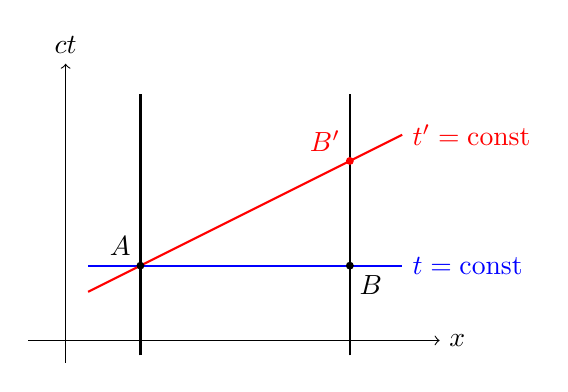
\begin{tikzpicture}[scale=.95]
\draw[->](-.5,0)--(5,0)node[right]{$x$};\draw[->](0,-.3)--(0,3.7)node[above]{$ct$};
\draw[thick](1,-.2)--(1,3.3);\draw[thick](3.8,-.2)--(3.8,3.3);
\draw[blue,thick](.3,1)--(4.5,1)node[right]{$t=\mathrm{const}$};
\draw[red,thick](.3,.65)--(4.5,2.75)node[right]{$t'=\mathrm{const}$};
\fill(1,1)circle(1.5pt)node[above left]{$A$};\fill(3.8,1)circle(1.5pt)node[below right]{$B$};
\fill[red](3.8,2.4)circle(1.5pt)node[above left]{$B'$};
\end{tikzpicture}}
图\ref{fv:o6:simultaneity}把杆画成在 $S$中静止的两条端点世界线。蓝线选出的 $A,B$满足 $\Delta t=0$；变换后却有 $\Delta t'=-\gamma V\Delta x/c^2\ne0$，不能用这对事件直接测量 $S'$中的杆长。$S'$的同时线满足 $ct=(V/c)x+\text{常量}$，应另选同一红线上两端的事件。长度收缩中的“同时测两端”，因而是选事件的条件，不是对同一对任意事件只作空间坐标变换。


图\ref{fv:o6:simultaneity}中杆在 $S$ 静止，故 $x_B-x_A=x_{B'}-x_A=L_0$。红线选取 $A,B'$，满足 $\Delta t'=0$，所以 $\Delta t=VL_0/c^2$。将它代入空间变换：
\[
 L'=\Delta x'=\gamma(L_0-V\Delta t)
 =\gamma L_0(1-\beta^2)=\frac{L_0}{\gamma}.
\]
这与前面“杆在 $S'$ 静止、在 $S$ 运动”的情形互为参照。每一方都在自己的同时线上选端点，所比较的是不同事件对，因而两方都测得对方的运动杆收缩并不矛盾。


\subsection{事件选择与测量条件}

每个测量量都对应特定的事件选择和参考系。时间膨胀选同一只钟的两次读数，长度收缩选测量系中同一时刻的两端，速度变换选同一粒子的相邻事件。对于爆炸、遮光、碰撞这类单个事件，应同时变换它的空间和时间坐标。
\begin{center}\small
\begin{tabular}{p{.20\textwidth}p{.32\textwidth}p{.34\textwidth}}
\toprule
所求量&所选事件或条件&可用关系\\\midrule
运动钟走时&同一随身钟经历两个事件&$\Delta t=\gamma\Delta\tau$\\
运动杆长度&测量系同时记录两端&$L=L_0/\gamma$\\
粒子速度&同一粒子上的相邻事件&$\dd x/\dd t$ 的洛伦兹变换\\
远处事件坐标&位置与时刻属于同一事件&同时变换 $x,t$\\
\bottomrule
\end{tabular}
\end{center}
例\ref{ex:hr5}和例\ref{ex:hr6}的不同“同时面”，以及练习\ref{hw:hr1}中跑道长度与赛跑位移的区别，都可先由这张表确定事件，再进行计算。

\section{两个光学实验}

\subsection{斐索实验与运动介质中的光速}

图\ref{fig:hrfizeau}表示干涉装置中两个等长水管的传播部分。两束光绕行方向相反，一束在两管内均顺水，另一束均逆水。令每管长度为 $l$，水速为 $V\ll c$，水静止系中的光速为 $c/n$，忽略色散。
\fig{fig:hrfizeau}{两管中的水流方向相反。两条互逆光路分别累计 $2l$ 的顺水路程和 $2l$ 的逆水路程。}{
\begin{tikzpicture}[scale=.85]
\fill[black!5](0,.6)rectangle(5,1.6);\fill[black!5](0,-1.6)rectangle(5,-.6);\draw(0,.6)rectangle(5,1.6);\draw(0,-1.6)rectangle(5,-.6);
\draw[ray](0,1)--(5,1);\draw[ray](5,1.3)--(0,1.3);\draw[ray](5,-1)--(0,-1);\draw[ray](0,-1.3)--(5,-1.3);
\draw[axis](1.5,2)--(3.5,2)node[midway,above]{$V$};\draw[axis](3.5,-2)--(1.5,-2)node[midway,below]{$V$};
\draw[aux](5,1)--(5.8,1)--(5.8,-1)--(5,-1);\draw[aux](0,1)--(-.8,1)--(-.8,-1)--(0,-1);
\node[left]at(-.8,0){分束与合束};\draw[dim](0,.15)--(5,.15)node[midway,above]{$l$};
\end{tikzpicture}}
对顺水传播，由前述速度变换得到
\[
u_+=\frac{c/n+V}{1+V/(nc)}
\simeq\frac cn+V\left(1-\frac1{n^2}\right).
\]
逆水速度的大小为 $|u_-|\simeq c/n-V(1-1/n^2)$。若以 $k=1-1/n^2$ 表示一阶系数，两束光的时间差为
\[
\Delta t=\frac{2l}{c/n-kV}-\frac{2l}{c/n+kV}
\simeq\frac{4lV(n^2-1)}{c^2}.
\]
该结果由介质系与装置系之间的速度变换得到，无须假设一种绝对静止的传播介质。

一阶展开中的两项都须保留。由 $(1+V/(nc))^{-1}\simeq1-V/(nc)$，
\[
\left(\frac cn+V\right)\left(1-\frac V{nc}\right)
=\frac cn+V-\frac V{n^2}+O(V^2/c).
\]
可见直接把 $c/n$ 与 $V$ 相加会漏掉 $-V/n^2$。在 $n\to1$ 的真空极限，两方向的速率都回到 $c$；在 $V\to0$ 时，则回到静止介质中的 $c/n$。这两个极限也能检查拖曳系数的形式。

\subsection{迈克耳孙—莫雷实验}

图\ref{fig:hrmichelson}中，两臂在装置静止系长度均为 $l$，分束镜 $M$ 将光分到 $M_1,M_2$，反射后在 $M$ 合束。
\fig{fig:hrmichelson}{等臂干涉仪。右臂平行于所假设的绝对运动方向，上臂与其垂直。}{
\begin{tikzpicture}
\draw[very thick](-.35,-.35)--(.35,.35);\draw[very thick](-.6,3)--(.6,3) (3,-.6)--(3,.6);
\draw[light](-2,0)--(0,0);\draw[light](.08,0)--(.08,3);\draw[light](-.08,3)--(-.08,0);\draw[light](0,.08)--(3,.08);\draw[light](3,-.08)--(0,-.08);\draw[light](0,0)--(0,-1.5);
\node[below left]at(0,0){$M$};\node[above]at(0,3){$M_1$};\node[right]at(3,0){$M_2$};\node[left]at(-2,0){$S$};\node[below]at(0,-1.5){$T$};
\draw[dim](-.9,0)--(-.9,3)node[midway,left]{$l$};\draw[dim](0,-.8)--(3,-.8)node[midway,below]{$l$};\draw[axis](1.2,2)--(3.2,2)node[right]{$V$};
\end{tikzpicture}}
按“相对绝对静止媒质光速为 $c$，装置作伽利略运动”的假设，平行臂与垂直臂的往返时间分别为
\[
t_\parallel=\frac l{c-V}+\frac l{c+V}
=\frac{2l/c}{1-\beta^2},\qquad
t_\perp=\frac{2l/c}{\sqrt{1-\beta^2}},\quad \beta=V/c.
\]
低速展开得 $t_\parallel-t_\perp\simeq l\beta^2/c$。装置转过 $90^\circ$ 后差值反号，预测的条纹移动为
\[
\Delta N\simeq\frac{2l}{\lambda}\frac{V^2}{c^2}.
\]
取 $l=11\,\mathrm m,V=3.0\times10^4\,\mathrm{m/s},\lambda=5.9\times10^{-7}\,\mathrm m$，预测约 $0.37$ 条。实验未出现这一预期的方向效应。狭义相对论在装置静止系直接给出两臂往返时间均为 $2l/c$，理想等臂装置转动后不会产生上述条纹移动。

上述预测是在一组特定假设下计算的：真空光相对某个绝对静止媒质各向同性，而装置的长度与时间又按经典规则处理。实验未出现预期的旋转效应，约束的是这组假设的共同预测，不能从结果单独推出“两束光都没有传播时间”或“仪器不发生干涉”。

图\ref{fig:hrmichelson}中，两臂往返相位差才决定条纹位置。旋转前若有固定的臂长误差，可能产生一个固定相位差；检验所关心的是旋转后随方向改变的那部分。在装置静止系使用相对论时，两臂的光速统一为 $c$，理想等臂的方向依赖自然消失，计算条件和观测量保持一致。

\section{动量、质量与能量}

\subsection{相对论动量与动能}

以下统一用 $m_0$ 表示粒子的不变质量，记其速度为 $u$，$\gamma_u=(1-u^2/c^2)^{-1/2}$。相对论动量、总能量为
\begin{equation}\label{eq:hrenergy}
\bm p=\gamma_um_0\bm u,\qquad E=\gamma_um_0c^2.
\end{equation}
若将 $E/c^2$ 另记为“动质量” $m_{\text{动}}$，则 $m_{\text{动}}=\gamma_um_0$，$\bm p=m_{\text{动}}\bm u$。这只是另一种记号；计算合成粒子的质量时，须明确所求的是不变质量，不能把各粒子的不变质量直接相加。

力定义为 $\bm F=\dd\bm p/\dd t$，功满足 $\dd K=\bm F\cdot\dd\bm r=\bm u\cdot\dd\bm p$。动能的计算以静止时 $K=0$为边界，积分结果记为
\begin{equation}\label{eq:hrkinetic}
\boxed{K=(\gamma_u-1)m_0c^2=E-m_0c^2.}
\end{equation}
对沿直线的运动，$p=m_0u/\sqrt{1-u^2/c^2}$，先对 $\gamma_u$ 使用链式法则：
\[
 \frac{\dd\gamma_u}{\dd u}
 =-\frac12(1-u^2/c^2)^{-3/2}\frac{-2u}{c^2}
 =\frac{u\gamma_u^3}{c^2}.
\]
再对 $p=m_0u\gamma_u$ 使用乘积法则，
\begin{align*}
 \frac{\dd p}{\dd u}
 &=m_0\left(\gamma_u+\frac{u^2}{c^2}\gamma_u^3\right)\\
 &=m_0\gamma_u^3\left(1-\frac{u^2}{c^2}+\frac{u^2}{c^2}\right)
 =m_0\gamma_u^3.
\end{align*}
于是 $\dd K=u\dd p=m_0u\gamma_u^3\dd u=m_0c^2\dd\gamma_u$。
静止时 $u=0$、$\gamma_u=1$、$K=0$，积分上下限一一对应：
\[
 \int_0^{K(u)}\dd K'
 =m_0c^2\int_1^{\gamma_u}\dd\gamma',
 \qquad K(u)=m_0c^2[\gamma']_1^{\gamma_u}
 =(\gamma_u-1)m_0c^2.
\]
这样得到式\eqref{eq:hrkinetic}，积分常量已由静止时的动能零点确定。同一微分关系还给出纵向运动的
\[
F=m_0\gamma_u^3\frac{\dd u}{\dd t}.
\]
因而实验室恒力并不对应恒加速度。粒子越快，同样的动量增量所造成的速度增量越小；继续做功主要使总能量和动量增长。

\fig{o6:momentum-energy-curves}{实线为相对论关系，虚线为经典近似；各图保持粒子不变质量相同}{\begin{tikzpicture}

\begin{scope}[x=4cm,y=.9cm]
\draw[axis](0,0)--(1.08,0)node[right]{$u/c$};
\draw[axis](0,0)--(0,3.4)node[above]{$p/(m_0c)$};
\draw[blue,thick,domain=0:.94,samples=100]plot(\x,{\x/sqrt(1-(\x)^2)});
\draw[dashed](0,0)--(.94,.94);
\node[below]at(1,0){$1$};\draw[aux](1,0)--(1,3.1);
\node[blue,left]at(.9,2.6){相对论};\node[above]at(.58,.58){经典};
\end{scope}
\begin{scope}[xshift=6.8cm,x=4cm,y=1.2cm]
\draw[axis](0,0)--(1.08,0)node[right]{$u/c$};
\draw[axis](0,0)--(0,2.55)node[above]{$K/(m_0c^2)$};
\draw[red,thick,domain=0:.94,samples=100]plot(\x,{1/sqrt(1-(\x)^2)-1});
\draw[dashed,domain=0:.94,samples=80]plot(\x,{.5*(\x)^2});
\node[below]at(1,0){$1$};\draw[aux](1,0)--(1,2.3);
\node[red,left]at(.9,1.7){相对论};\node[above]at(.63,.2){经典};
\end{scope}

\end{tikzpicture}}
图\ref{o6:momentum-energy-curves}中，两种关系在 $u/c\ll1$ 时接近；接近光速时，实线的动量和动能都急剧增大。对有质量粒子，$u\to c^-$ 要求无界的能量，有限做功不能使它达到或越过 $c$。图中低速近似的抛物线不能向高速无限外推。

低速展开 $\gamma_u\simeq1+u^2/(2c^2)$，才退化为 $K\simeq m_0u^2/2$。恒力对应动量随时间线性增长，速度却不会随时间无限增大，例\ref{ex:hr11}将具体计算。

\subsection{换参考系时的能量与动量}

总能量、动量分别依赖参考系，但同一系统的不变质量不依赖参考系。设 $S'$ 相对 $S$ 沿 $+x$ 以速度 $V$ 运动。将速度变换代入 $E=\gamma_um_0c^2$、$p_x=\gamma_um_0u_x$，利用
\[
 \gamma_{u'}=\gamma_V\gamma_u\left(1-\frac{Vu_x}{c^2}\right),
\]
得到
\[
 E'=\gamma_V(E-Vp_x),\qquad
 p_x'=\gamma_V\left(p_x-\frac{VE}{c^2}\right),\qquad
 p_y'=p_y,\quad p_z'=p_z.
\]
这些关系是线性的，对各粒子相加后仍成立，所以也可变换整个碰撞系统的总能量与总动量。不能把 $S$ 系的动能与 $S'$ 系的动量放入同一质量公式，也不能只变换入射粒子而让靶粒子在两系中都保持静止。

若在 $S$ 系有 $E_{\text{初}}=E_{\text{末}}$、$\bm P_{\text{初}}=\bm P_{\text{末}}$，代入上述线性关系便同时得到 $S'$ 系的两条守恒式。守恒不表示数值在不同系中相同，而是同一系内的初、末总量相同。比较一个碰撞前后时，先固定参考系，再逐项列出参与物体；需要换系时，将所有参与物体一起变换。

\subsection{能量动量关系与守恒}

消去 $\gamma_u,u$，得到
\begin{equation}\label{eq:hrem}
\boxed{E^2-p^2c^2=m_0^2c^4,\qquad \bm u=\frac{c^2\bm p}{E}.}
\end{equation}
式\eqref{eq:hrem}可直接从同一粒子的能量、动量求出：
\[
 E^2-p^2c^2=\gamma_u^2m_0^2c^4(1-u^2/c^2)=m_0^2c^4.
\]
\fig{o6:mass-hyperbola}{同一有质量粒子在不同参考系中的能量、动量数值落在同一正能量双曲线上}{\begin{tikzpicture}

\begin{scope}[x=1.1cm,y=1.1cm]
\draw[axis](-2.8,0)--(3,0)node[right]{$p_x/(m_0c)$};
\draw[axis](0,-.2)--(0,3.4)node[above]{$E/(m_0c^2)$};
\draw[gray,dashed](-2.7,2.7)--(0,0)--(2.7,2.7);
\draw[thick,domain=-2.5:2.5,samples=120]plot(\x,{sqrt(1+(\x)^2)});
\fill[blue](1.732051,2)circle(1.6pt)node[right]{$S:(\sqrt3,2)$};
\fill[red](0,1)circle(1.6pt)node[below left]{$S':(0,1)$};
\draw[axis,blue](1.45,1.95)..controls(.9,1.4)and(.55,1.22)..(.2,1.12);
\node[above]at(0,4.2){$E^2-p_x^2c^2=m_0^2c^4$};
\end{scope}

\end{tikzpicture}}
图\ref{o6:mass-hyperbola}只考虑沿 $x$ 的运动。在 $S$ 中取 $E=2m_0c^2,p_x=\sqrt3m_0c$，则粒子速度为 $u=\sqrt3c/2$；选 $V=u$ 变到粒子静止系后，$p'_x=0,E'=m_0c^2$。能量与动量都改变，双曲线所代表的不变质量保持不变。灰虚线对应 $E=|p_x|c$，有质量粒子的数值位于其上方。

光子的 $m_0=0$，故 $E=pc=h\nu=hc/\lambda$。光子有能量和动量，没有可供选取的静止参考系。

孤立系统的总能量、总动量守恒。把整个系统视为一个整体，其不变质量 $M$ 由
\[
M^2c^4=E_{\text{总}}^2-c^2|\bm p_{\text{总}}|^2
\]
确定。完全非弹性碰撞中，部分相对运动能转化为复合物的内能，所以 $M$ 可以大于碰前各粒子不变质量之和。衰变、光子反冲和康普顿散射也应同时使用能量、动量守恒。

守恒式中的系统边界须一致。若末态有复合粒子和辐射，二者都应列入：
\[
\sum E_{\text{初}}=E_{\text{复合}}+E_{\text{辐射}},\qquad
\sum\bm p_{\text{初}}=\bm p_{\text{复合}}+\bm p_{\text{辐射}}.
\]
只有初态总动量为零且末态没有外逸动量时，复合粒子才在该系静止，才能直接以 $Mc^2$ 表示它的全部能量。若总动量 $\bm P\ne0$，则先由 $E_{\text{总}}^2-P^2c^2$ 求系统不变质量；若 $M>0$，系统整体静止系相对当前系的速度为 $\bm V_{\rm cm}=c^2\bm P/E_{\text{总}}$，其大小严格小于 $c$。当 $M=0$ 且总能量非零时，该表达式的大小为 $c$，不对应可选取的惯性静止系。

\fig{fig:hr-photon-system}{两个光子的单独静质量均为零，合系统的静质量仍取决于夹角。左图反向等能，总动量为零；右图同向，总动量为 $2E_\gamma/c$。}{
\begin{tikzpicture}[scale=.9]
\fill(0,0)circle(1.5pt);\draw[light](0,0)--(-2.3,0)node[above]{$E_\gamma$};\draw[light](0,0)--(2.3,0)node[above]{$E_\gamma$};\node[below]at(0,-.55){$M=2E_\gamma/c^2$};
\begin{scope}[shift={(6.6,0)}]\draw[light](0,.3)--(2.8,.3)node[right]{$E_\gamma$};\draw[light](0,-.3)--(2.8,-.3)node[right]{$E_\gamma$};\node[below]at(1.4,-.8){$M=0$};\end{scope}
\end{tikzpicture}}
图\ref{fig:hr-photon-system}可由 $E_\gamma=pc$ 直接验证。一般两个光子有
\[
M^2c^4=2E_1E_2(1-\cos\theta).
\]
同向时整体仍没有静止系；反向等能时则有静止系，能量全部计入系统静能。这说明“各粒子的静质量相加”与“求整个系统的静质量”是不同的运算。练习\ref{hw:hr5}将用这一关系反推母粒子的质量。

\section{非惯性系、局部引力与时钟}

\subsection{惯性力与等效原理}

在低速近似下，相对于惯性系做平动加速的参考系中，可以引入惯性力 $\bm F_{\mathrm{in}}=-m_{\mathrm i}\bm a$，使运动方程保持通常的形式。引力中的 $m_{\mathrm g}$ 决定物体受到的引力，惯性质量 $m_{\mathrm i}$ 则决定物体对加速的响应。自由落体加速度与物体组成无关，表明二者成比例；采用通常的单位约定可令 $m_{\mathrm g}=m_{\mathrm i}$。

图\ref{fig:hr-gr1}比较一个向上加速的小舱和一个处于引力场中的小舱。对足够小的空间区域和足够短的时间，舱内实验不能区分均匀引力与相应的加速效应。这是等效原理的局部表述。
\fig{fig:hr-gr1}{小舱内的加速效应与局部引力效应}{
\begin{tikzpicture}[scale=.9]
\draw[world](0,0)rectangle(3,3);\fill(1.5,1.5)circle(3pt);\draw[axis](1.5,1.4)--(1.5,.5)node[right]{$m\bm g$};\draw[axis](-.5,2.6)--(-.5,1.4)node[left]{$\bm g$};\node at(1.5,-.5){引力场中的小舱};
\begin{scope}[shift={(6,0)}]
\draw[world](0,0)rectangle(3,3);\fill(1.5,1.5)circle(3pt);\draw[axis](1.5,1.4)--(1.5,.5)node[right]{$-m\bm a$};\draw[axis](3.6,1.4)--(3.6,2.6)node[right]{$\bm a$};\node at(1.5,-.5){远离引力场的加速舱};
\end{scope}
\end{tikzpicture}}
局部条件不可省略。跨越较大区域时，引力方向和大小可能随位置变化，产生潮汐效应；一个整体平动加速的参考系不能消去这些变化。

\subsection{轨道、光线与时钟}

广义相对论用时空几何描述引力，可以计算行星轨道的相对论修正、掠过天体的光线偏折，以及不同高度时钟的速率差。这里先给出弱场、低速情形下的时钟关系。

对静止于弱引力场中的时钟，若 $\Phi$ 为引力势且 $|\Phi|/c^2\ll1$，则
\[
\dd\tau\simeq\left(1+\frac{\Phi}{c^2}\right)\dd t.
\]
比较图\ref{fig:hr-gr2}中的上下两处，$\Phi_2>\Phi_1$，高处时钟相对于低处走得较快。低处发出的光到达高处后，由高处本地时钟测得的频率降低，近似满足
\[
\frac{\nu_2-\nu_1}{\nu_1}\simeq-\frac{\Phi_2-\Phi_1}{c^2}.
\]
\fig{fig:hr-gr2}{静态弱引力场中的时钟比较与向上传播的光}{
\begin{tikzpicture}[scale=.95]
\draw[world](-.5,0)--(6.5,0);\draw[world](-.5,2.5)--(6.5,2.5);\draw[axis](-1.1,2)--(-1.1,.5)node[midway,left]{$\bm g$};
\draw[world](0,0)circle(.3);\node[above right]at(.5,0){$\Phi_1,\ \nu_1$};\draw[world](0,2.5)circle(.3);\node[above right]at(.5,2.5){$\Phi_2>\Phi_1,\ \nu_2<\nu_1$};
\draw[light](4.7,.2)--(4.7,2.3)node[midway,right]{光向上传播};
\end{tikzpicture}}
引力势决定上述时钟比较，不能仅凭某一点的引力场强大小判断时钟快慢。狭义相对论的运动学效应与引力效应在实际比较中还可能同时出现。
例如在地面附近取较小高度差 $h$，近似有 $\Phi_2-\Phi_1\simeq gh$，于是
\[
\frac{\dd\tau_2}{\dd\tau_1}\simeq1+\frac{gh}{c^2},\qquad
\frac{\nu_2-\nu_1}{\nu_1}\simeq-\frac{gh}{c^2}.
\]
频率变化的符号也可从波峰计数理解。静态场中，连续两波峰到达上下两处的坐标时间间隔相同，记为 $\dd t$；本地测得的周期却分别为 $\dd\tau_1,\dd\tau_2$。因而
\[
 \frac{\nu_2}{\nu_1}=\frac{\dd\tau_1}{\dd\tau_2}
 \simeq\frac{1+\Phi_1/c^2}{1+\Phi_2/c^2}
 \simeq1-\frac{\Phi_2-\Phi_1}{c^2}.
\]
频率比较必须使用各处本地钟，而不能把两个位置的固有时间先当成相同。

图\ref{fig:hr-gr2}的上方时钟每一单位坐标时间走得稍快，向上传播的光在上方用本地钟计量时频率稍低；两个符号描述的是同一次比较的不同测量量。这里要求静态弱场、上下两处相对静止，且高度范围内 $g$ 的变化可以忽略。

引力场的扰动也能以波的形式传播。引力波在局部表现为横向两个方向上交替的潮汐伸缩，可通过比较互相垂直的光程变化进行测量。理解这类现象需要把本讲的时钟、光信号和事件观点推广到弯曲时空。
